\section {R computations}
If you are completely new to programming, the R prompt will demonstrate a few basics. Here we define \(x\) and adds 3 to it:

\begin{rscript}
> x=5
> x+3
[1] 8
\end{rscript}

While some operations are intuitive others require getting used to. For example, the hat ($\wedge$) exponentiates and double-percentage (\code{\%\%}) finds the remainder of a division:

\begin{rscript}
> x^2 $a^x$
[1] 25
> x%\%\%%3
[1] 2
> x^2%\%\%%7
[1] 4
\end{rscript}

Long computations should be broken into smaller steps. In R this is achieved by defining functions. Here, we defined a function called \code{mouse}. It takes a number as input and outputs half of that number (if it was even) or three times the number plus 1 (if it was uneven):

\begin{rscript}
> mouse = function(n) if (n%\%\%2%==0) n/2 else 3*n+1
> mouse(8)
[1] 4
> mouse(9)
[1] 28
\end{rscript}

You can create large models in this way in R but R does not scale well to complexity. Soon you are over your head in code. Yet, R remains an important tool for the modeller because it is very easy to develop and test small pieces of a model in R. These small pieces can then be transferred into \CPP\ code using the \US\ framework.

\section {\US\ computations}
\label{ch:computations-us-computations}
When you run a box script, you will notice from the feedback on the screen, that \US\ goes through a number of steps:
\medskip
\begin{compactenum}
\item Construct all boxes
\item Amend all boxes
\item Run root box
\begin{compactenum}
  \item Initialize
  \item Reset
  \item Update
  \item Cleanup
  \item Debrief
\end{compactenum}
\end{compactenum}
\medskip

These steps serve different  purposes. Each have a certain role when  defining the behaviour for a certain class of boxes, such as \code{Stage} or \code{DayDegree}. 

Any box needs to be created (step 1) but the following steps are optional. The purpose of amending (step 2) is to create additional boxes and ports, not defined in the box script, but in the \CPP\ code. This is an advanced technique that can be used, for example, to spawn hundreds or thousands of \code{Box} objects in spatially-explicit or metapopulation models.

For the generic \code{Box} base class, these steps all default to do nothing. In effect you have a box void of any functionality. To create a new class of boxes with some desired functionality, you derive the new class from \code{Box} in \CPP\ using \code{Box} as the base class. This is an object-oriented mechanism known as  inheritance.

While box construction is carried out by the constructor method in \CPP, the remaining steps have a corresponding virtual function. To code the update step, for example, you write \CPP\ code for the \code{update} method of your class.

When you issue the \uscom{load} command at the \US\ prompt, all boxes defined in the box script will be created and amended (steps 1-2). With the \uscom{run} command, all three steps (1-3) are carried out so, in addition, the root box will be run (step 3). 

The root box is the outermost box in the script, containing all the other boxes. The root box, usually a \code{Simulation} box, governs the execution of the subsequent steps (3a-3e). As depicted in \iref{fig:computation-steps}, the \code{Simulation} box executes these steps in a double loop: \code{Simulation}'s \code{iterations} input determines the number of steps in the outer loop, and its \code{steps} input determines the number of steps in the inner loop.

For example, you could set \code{steps} to 365, if you wanted to run a simulation for 365 time steps. The \code{update} method would then be called 365 times, with the \code{reset} called once at first and \code{cleanup} called once at last.

If you wanted the whole simulation repeated 10 times (\eg\ to simulate different scenarios)  you would set \code{iterations} to 10. The whole inner loop (\code{reset} once--\code{update} many times--\code{cleanup} once) would then be executed 10 times, with \code{initialize} called once at first and \code{debrief} called once at last. The \code{iterations} input defaults to a value of 1. 

In practice, for most boxes it suffices to define their \code{reset} and \code{update} methods to code their behaviour, in addition to their constructor which is mandatory in \CPP.
 
\begin{figure}
\centering
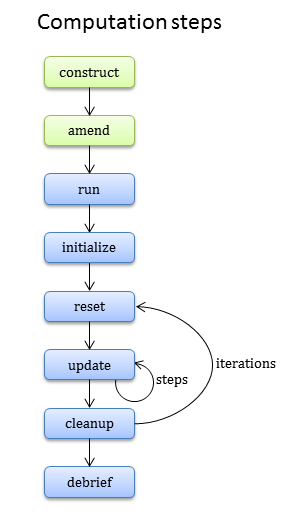
\includegraphics[scale=0.8]{graphics/computation-steps}
\caption{The computation steps in \US. Green steps are carried out when a box script is loaded. Blue steps are carried out, in addition to the green steps, when the script is run.}
\label{fig:computation-steps}
\end{figure}

Since a box script usually consists of more than one box, \code{Simulation} needs a rule to determine in which order to process (\eg\ update) the boxes. The rule has two parts:
\medskip
\begin{compactenum}
\item Top to bottom
\item Always children first
\end{compactenum}
\medskip

Let's revisit the \filenameexplained{book/egg5.box} script and figure out, in which order the boxes are processed (\iref{fig:box-tree}).
\begin{figure}
\centering
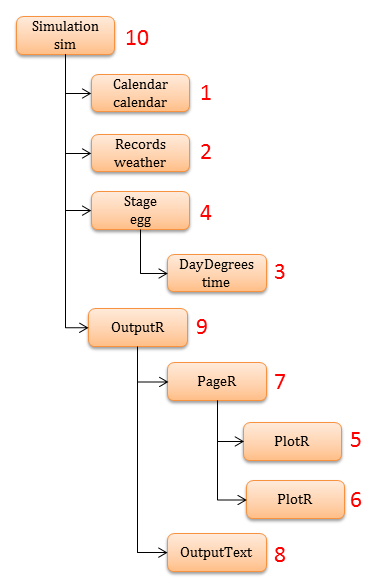
\includegraphics[scale=0.8]{graphics/box-tree}
\caption{The computation order (numbered 1 to 10 in red) of the boxes found in \filename{\ushome/book/egg5.box}.}
\label{fig:box-tree}
\end{figure}

The computation order is important for boxes that depend on input produced by other boxes another box. In this example (\iref{fig:box-tree}), for example, \code{calendar} is the first box processed in any step. This makes sense because it keeps track of the current date (available in its \code{date} output), and other boxes are likely to depend on knowing the date of the current time step.
